\documentclass[tikz,border=6pt]{standalone}
\usepackage{ctex}
\usepackage{amsmath}
\usetikzlibrary{calc, arrows.meta}

\begin{document}
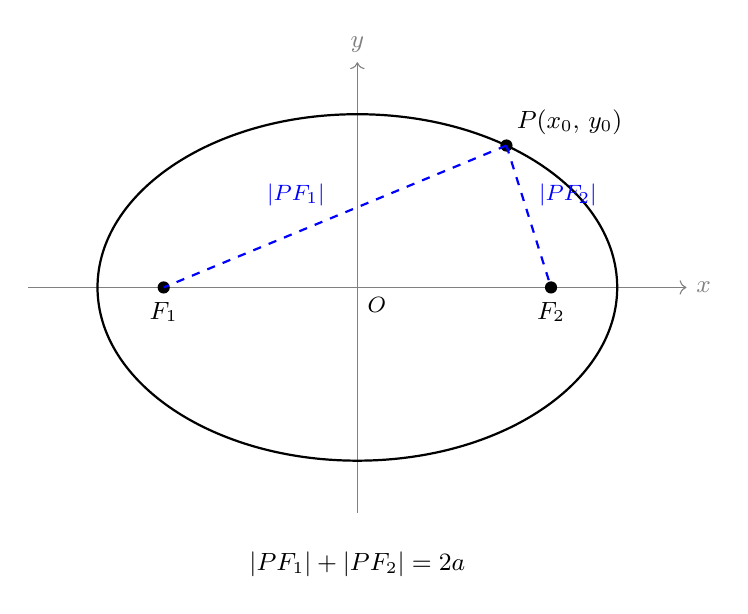
\begin{tikzpicture}[scale=1.1, thick]

% 椭圆：a=3, b=2, c=sqrt(5)≈2.236
% 焦点在 x 轴：F1=(-sqrt(5),0), F2=(sqrt(5),0)

% 坐标轴
\draw[->, thin, gray] (-3.8, 0) -- (3.8, 0) node[right, font=\small] {$x$};
\draw[->, thin, gray] (0, -2.6) -- (0, 2.6) node[above, font=\small] {$y$};
\node[font=\footnotesize, below right] at (0,0) {$O$};

% 椭圆
\draw[black, thick] (0,0) ellipse (3 and 2);

% 焦点 F1, F2
\fill[black] ({-sqrt(5)}, 0) circle [radius=2pt];
\fill[black] ({sqrt(5)}, 0) circle [radius=2pt];
\node[font=\small, below] at ({-sqrt(5)}, -0.05) {$F_1$};
\node[font=\small, below] at ({sqrt(5)}, -0.05) {$F_2$};

% 动点 P（在椭圆上的第一象限点，取角度约55°）
\coordinate (P) at ({3*cos(55)}, {2*sin(55)});
\fill[black] (P) circle [radius=2pt];
\node[above right, font=\small] at (P) {$P(x_0,\,y_0)$};

% 焦半径 PF1, PF2（蓝色虚线）
\draw[blue, dashed, thick] (P) -- ({-sqrt(5)}, 0) node[midway, above left, font=\footnotesize] {$|PF_1|$};
\draw[blue, dashed, thick] (P) -- ({sqrt(5)}, 0) node[midway, above right, font=\footnotesize] {$|PF_2|$};

% 标注：|PF1|+|PF2|=2a
\node[font=\small, align=center] at (0, -3.2)
  {$|PF_1| + |PF_2| = 2a$};

\end{tikzpicture}
\end{document}
